\documentclass{article}

% Packages required by doxygen
\usepackage{calc}
\usepackage{doxygen}
\usepackage{graphicx}
\usepackage[utf8]{inputenc}
\usepackage{makeidx}
\usepackage{multicol}
\usepackage{multirow}
\usepackage{textcomp}
\usepackage[table]{xcolor}

% NLS support packages
\usepackage{polski}
\usepackage[T1]{fontenc}

% Font selection
\usepackage[T1]{fontenc}
\usepackage{mathptmx}
\usepackage[scaled=.90]{helvet}
\usepackage{courier}
\usepackage{amssymb}
\usepackage{sectsty}
\renewcommand{\familydefault}{\sfdefault}
\allsectionsfont{%
  \fontseries{bc}\selectfont%
  \color{darkgray}%
}
\renewcommand{\DoxyLabelFont}{%
  \fontseries{bc}\selectfont%
  \color{darkgray}%
}

% Page & text layout
\usepackage{geometry}
\geometry{%
  a4paper,%
  top=2.5cm,%
  bottom=2.5cm,%
  left=2.5cm,%
  right=2.5cm%
}
\tolerance=750
\hfuzz=15pt
\hbadness=750
\setlength{\emergencystretch}{15pt}
\setlength{\parindent}{0cm}
\setlength{\parskip}{0.2cm}
\makeatletter
\renewcommand{\paragraph}{%
  \@startsection{paragraph}{4}{0ex}{-1.0ex}{1.0ex}{%
    \normalfont\normalsize\bfseries\SS@parafont%
  }%
}
\renewcommand{\subparagraph}{%
  \@startsection{subparagraph}{5}{0ex}{-1.0ex}{1.0ex}{%
    \normalfont\normalsize\bfseries\SS@subparafont%
  }%
}
\makeatother

% Headers & footers
\usepackage{fancyhdr}
\pagestyle{fancyplain}
\fancyhead[LE]{\fancyplain{}{\bfseries\thepage}}
\fancyhead[CE]{\fancyplain{}{}}
\fancyhead[RE]{\fancyplain{}{\bfseries\leftmark}}
\fancyhead[LO]{\fancyplain{}{\bfseries\rightmark}}
\fancyhead[CO]{\fancyplain{}{}}
\fancyhead[RO]{\fancyplain{}{\bfseries\thepage}}
\fancyfoot[LE]{\fancyplain{}{}}
\fancyfoot[CE]{\fancyplain{}{}}
\fancyfoot[RE]{\fancyplain{}{\bfseries\scriptsize Wygenerowano Śr, 25 mar 2015 14\-:41\-:17 dla Lab03 -\/ podstawowe struktury danych\-: tablice programem Doxygen }}
\fancyfoot[LO]{\fancyplain{}{\bfseries\scriptsize Wygenerowano Śr, 25 mar 2015 14\-:41\-:17 dla Lab03 -\/ podstawowe struktury danych\-: tablice programem Doxygen }}
\fancyfoot[CO]{\fancyplain{}{}}
\fancyfoot[RO]{\fancyplain{}{}}
\renewcommand{\footrulewidth}{0.4pt}
\renewcommand{\chaptermark}[1]{%
  \markboth{#1}{}%
}
\renewcommand{\sectionmark}[1]{%
  \markright{\thesection\ #1}%
}

% Indices & bibliography
\usepackage{natbib}
\usepackage[titles]{tocloft}
\setcounter{tocdepth}{3}
\setcounter{secnumdepth}{5}
\makeindex

% Hyperlinks (required, but should be loaded last)
\usepackage{ifpdf}
\ifpdf
  \usepackage[pdftex,pagebackref=true]{hyperref}
\else
  \usepackage[ps2pdf,pagebackref=true]{hyperref}
\fi
\hypersetup{%
  colorlinks=true,%
  linkcolor=blue,%
  citecolor=blue,%
  unicode%
}

% Custom commands
\newcommand{\clearemptydoublepage}{%
  \newpage{\pagestyle{empty}\cleardoublepage}%
}


%===== C O N T E N T S =====

\begin{document}

% Titlepage & ToC
\hypersetup{pageanchor=false}
\pagenumbering{roman}
\begin{titlepage}
\vspace*{7cm}
\begin{center}%
{\Large Lab03 -\/ podstawowe struktury danych\-: tablice }\\
\vspace*{1cm}
{\large Mateusz Krawczuk, nr indeksu 209147}\\
\vspace{0.5cm}
{\large Wygenerowano przez Doxygen 1.8.6}\\
\vspace*{0.5cm}
{\small Śr, 25 mar 2015 14:41:17}\\
\end{center}
\end{titlepage}
%\clearemptydoublepage
%\tableofcontents
%\clearemptydoublepage
\pagenumbering{arabic}
%\hypersetup{pageanchor=true}

%--- Begin generated contents ---
\part{Streszczenie}
Niniejszy dokument zawiera wyniki pomiaru czasu, którego potrzebował mój komputer na wykonanie operacji mnożenia przez 2 na zestawach danych o długościach od 1 do 10e8 elementów. Zawiera także dokumentację kodu programu użytego do wykonania tego badania.

\part{Sprawozdanie}
Obliczenia wykonano na 64-bitowym procesorze AMD Athlon X2. Wykres przedstawia zależność czasu wykonywania operacji od długości ciągu danych. Został wygenerowany za pomocą Gnuplota. Podziałki na obydwu osiach są w skali logarytmicznej. Na wykresie umieszczono także prostą y = (0.7803/10e8)x. Dzięki temu lepiej widać, że jest to zależność mocno zbliżona do liniowej - można na tej podstawie domniemywać, że złożoność obliczeniowa tej operacji jest O(n). Warto zwrócić uwagę na długość wykonywania operacji na jednym elemencie danych - przewyższa on o rząd wielkości czas wykonywania na dziesięciu elementach.
\centerline{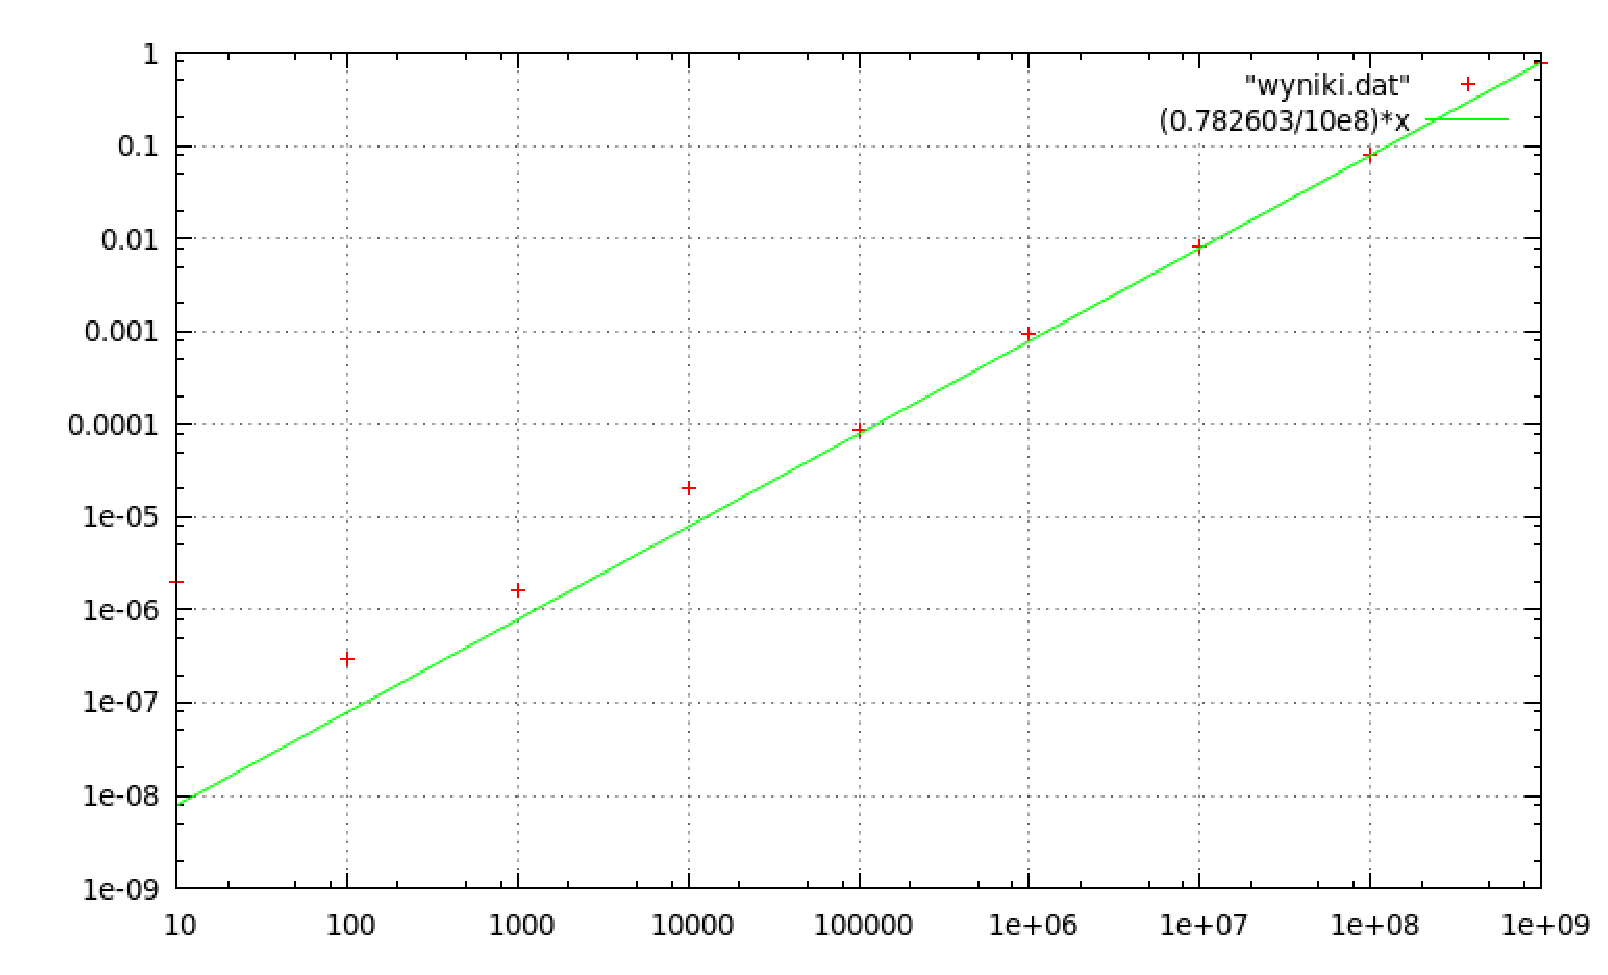
\includegraphics[width=\textwidth,height=\textheight,keepaspectratio]{wykres1.eps}}

\part{Dokumentacja przestrzeni nazw}
\hypertarget{namespacearr}{\section{Dokumentacja przestrzeni nazw arr}
\label{namespacearr}\index{arr@{arr}}
}
\subsection*{Komponenty}
\begin{DoxyCompactItemize}
\item 
class \hyperlink{classarr_1_1_kolejka}{Kolejka}
\item 
class \hyperlink{classarr_1_1_lista}{Lista}
\item 
class \hyperlink{classarr_1_1_stos}{Stos}
\end{DoxyCompactItemize}

\hypertarget{namespacels}{\section{Dokumentacja przestrzeni nazw ls}
\label{namespacels}\index{ls@{ls}}
}


\hyperlink{classls_1_1_kolejka}{Kolejka}, abstrakcyjna struktura danych z buforem typu L\-I\-F\-O.  


\subsection*{Komponenty}
\begin{DoxyCompactItemize}
\item 
class \hyperlink{classls_1_1_kolejka}{Kolejka}
\item 
class \hyperlink{classls_1_1_kontener}{Kontener}
\item 
class \hyperlink{classls_1_1_stos}{Stos}
\end{DoxyCompactItemize}


\subsection{Opis szczegółowy}
\hyperlink{classls_1_1_stos}{Stos}, abstrakcyjna struktura danych z buforem typu F\-I\-F\-O. 
\part{Dokumentacja klas}
\hypertarget{classls_1_1_kolejka}{\section{Dokumentacja klasy ls\-:\-:Kolejka}
\label{classls_1_1_kolejka}\index{ls\-::\-Kolejka@{ls\-::\-Kolejka}}
}


{\ttfamily \#include $<$kolejka.\-h$>$}

Diagram dziedziczenia dla ls\-:\-:Kolejka\begin{figure}[H]
\begin{center}
\leavevmode
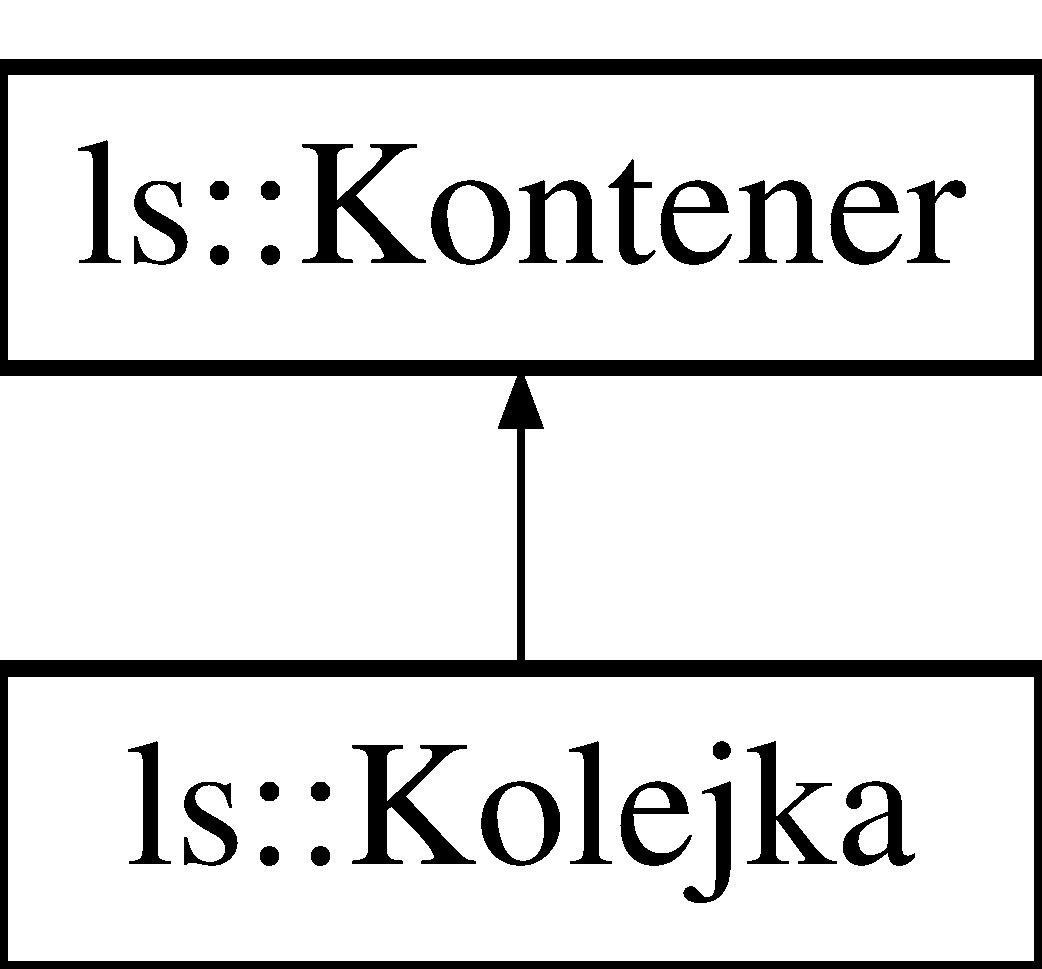
\includegraphics[height=2.000000cm]{classls_1_1_kolejka}
\end{center}
\end{figure}
\subsection*{Metody publiczne}
\begin{DoxyCompactItemize}
\item 
int \hyperlink{classls_1_1_kolejka_ac11693677f596b8a6dd2fc0183bbde90}{pop} ()
\begin{DoxyCompactList}\small\item\em Pop kolejki jaki jest, każdy widzi. Usuwa najstarszy element i zwraca wartość przez niego przechowywaną. \end{DoxyCompactList}\end{DoxyCompactItemize}
\subsection*{Dodatkowe Dziedziczone Składowe}


\subsection{Opis szczegółowy}


Definicja w linii 14 pliku kolejka.\-h.



\subsection{Dokumentacja funkcji składowych}
\hypertarget{classls_1_1_kolejka_ac11693677f596b8a6dd2fc0183bbde90}{\index{ls\-::\-Kolejka@{ls\-::\-Kolejka}!pop@{pop}}
\index{pop@{pop}!ls::Kolejka@{ls\-::\-Kolejka}}
\subsubsection[{pop}]{\setlength{\rightskip}{0pt plus 5cm}int ls\-::\-Kolejka\-::pop (
\begin{DoxyParamCaption}
{}
\end{DoxyParamCaption}
)\hspace{0.3cm}{\ttfamily [inline]}}}\label{classls_1_1_kolejka_ac11693677f596b8a6dd2fc0183bbde90}


Definicja w linii 21 pliku kolejka.\-h.



Dokumentacja dla tej klasy została wygenerowana z pliku\-:\begin{DoxyCompactItemize}
\item 
\hyperlink{kolejka_8h}{kolejka.\-h}\end{DoxyCompactItemize}

\hypertarget{classarr_1_1_kolejka}{\section{Dokumentacja klasy arr\-:\-:Kolejka}
\label{classarr_1_1_kolejka}\index{arr\-::\-Kolejka@{arr\-::\-Kolejka}}
}


{\ttfamily \#include $<$kolejka\-\_\-arr.\-h$>$}

\subsection*{Metody publiczne}
\begin{DoxyCompactItemize}
\item 
\hyperlink{classarr_1_1_kolejka_a7f2d0e05c25b3a0d10db8e04cd4bdb58}{Kolejka} ()
\begin{DoxyCompactList}\small\item\em Konstruktor domyślny klasy \hyperlink{classarr_1_1_kolejka}{arr\-::\-Kolejka}. \end{DoxyCompactList}\item 
\hyperlink{classarr_1_1_kolejka_a1addd7f5fdee63f093fd971037600b02}{Kolejka} (const \hyperlink{classarr_1_1_kolejka}{Kolejka} \&lewy)
\begin{DoxyCompactList}\small\item\em Konstruktor kopiujący klasy \hyperlink{classarr_1_1_kolejka}{arr\-::\-Kolejka}. \end{DoxyCompactList}\item 
\hyperlink{classarr_1_1_kolejka_a455a5aac4ea9612cab749b8e9edf131d}{$\sim$\-Kolejka} ()
\begin{DoxyCompactList}\small\item\em Destruktor klasy \hyperlink{classarr_1_1_kolejka}{arr\-::\-Kolejka}. \end{DoxyCompactList}\item 
void \hyperlink{classarr_1_1_kolejka_acb08e887411da797ab39960cde892dc5}{push} (int val)
\begin{DoxyCompactList}\small\item\em Wrzuca element na szczyt kolejki. \end{DoxyCompactList}\item 
int \hyperlink{classarr_1_1_kolejka_a9d2c0676d6992ffb3b2aa4cd27ca36af}{pop} ()
\begin{DoxyCompactList}\small\item\em Zdejmuje najstarszy element z kolejki. \end{DoxyCompactList}\item 
bool \hyperlink{classarr_1_1_kolejka_a8ed4d617d36bf539544d1f7e18929bf8}{empty} ()
\begin{DoxyCompactList}\small\item\em Sprawdza, czy kolejka jest pusta. \end{DoxyCompactList}\item 
int \hyperlink{classarr_1_1_kolejka_a1aabde2dffcb50f4d8dc2e7d6df808ce}{size} ()
\begin{DoxyCompactList}\small\item\em Zwraca rozmiar kolejki. \end{DoxyCompactList}\end{DoxyCompactItemize}
\subsection*{Metody prywatne}
\begin{DoxyCompactItemize}
\item 
void \hyperlink{classarr_1_1_kolejka_affc094df5944c66cecfcaaeb490b7d67}{rozszerz\-\_\-x2} ()
\begin{DoxyCompactList}\small\item\em Metoda zwiększa dwukrotnie pojemnosć kolejki. \end{DoxyCompactList}\item 
void \hyperlink{classarr_1_1_kolejka_a05e15597ec59b3c77ba15112b4018b2f}{rozszerz\-\_\-1} ()
\begin{DoxyCompactList}\small\item\em Metoda zwiększa pojemnosć kolejki o 1. \end{DoxyCompactList}\end{DoxyCompactItemize}
\subsection*{Atrybuty prywatne}
\begin{DoxyCompactItemize}
\item 
int $\ast$ \hyperlink{classarr_1_1_kolejka_a80a504c56893e43ae1b407b971b501a7}{tablica}
\item 
int \hyperlink{classarr_1_1_kolejka_adbfdaca50c2b0bbe75d9b1e572f9b320}{rozmiar\-\_\-kol}
\item 
int \hyperlink{classarr_1_1_kolejka_ae10930beaa121ee5b178ffbb10b175e7}{pojemnosc\-\_\-kol}
\end{DoxyCompactItemize}


\subsection{Opis szczegółowy}


Definicja w linii 7 pliku kolejka\-\_\-arr.\-h.



\subsection{Dokumentacja konstruktora i destruktora}
\hypertarget{classarr_1_1_kolejka_a7f2d0e05c25b3a0d10db8e04cd4bdb58}{\index{arr\-::\-Kolejka@{arr\-::\-Kolejka}!Kolejka@{Kolejka}}
\index{Kolejka@{Kolejka}!arr::Kolejka@{arr\-::\-Kolejka}}
\subsubsection[{Kolejka}]{\setlength{\rightskip}{0pt plus 5cm}arr\-::\-Kolejka\-::\-Kolejka (
\begin{DoxyParamCaption}
{}
\end{DoxyParamCaption}
)\hspace{0.3cm}{\ttfamily [inline]}}}\label{classarr_1_1_kolejka_a7f2d0e05c25b3a0d10db8e04cd4bdb58}


Definicja w linii 26 pliku kolejka\-\_\-arr.\-h.

\hypertarget{classarr_1_1_kolejka_a1addd7f5fdee63f093fd971037600b02}{\index{arr\-::\-Kolejka@{arr\-::\-Kolejka}!Kolejka@{Kolejka}}
\index{Kolejka@{Kolejka}!arr::Kolejka@{arr\-::\-Kolejka}}
\subsubsection[{Kolejka}]{\setlength{\rightskip}{0pt plus 5cm}arr\-::\-Kolejka\-::\-Kolejka (
\begin{DoxyParamCaption}
\item[{const {\bf Kolejka} \&}]{lewy}
\end{DoxyParamCaption}
)}}\label{classarr_1_1_kolejka_a1addd7f5fdee63f093fd971037600b02}
Bezużyteczny dla trzeciego zadania, ale na pewno kolega się ucieszy. 

Definicja w linii 3 pliku kolejka\-\_\-arr.\-cpp.

\hypertarget{classarr_1_1_kolejka_a455a5aac4ea9612cab749b8e9edf131d}{\index{arr\-::\-Kolejka@{arr\-::\-Kolejka}!$\sim$\-Kolejka@{$\sim$\-Kolejka}}
\index{$\sim$\-Kolejka@{$\sim$\-Kolejka}!arr::Kolejka@{arr\-::\-Kolejka}}
\subsubsection[{$\sim$\-Kolejka}]{\setlength{\rightskip}{0pt plus 5cm}arr\-::\-Kolejka\-::$\sim$\-Kolejka (
\begin{DoxyParamCaption}
{}
\end{DoxyParamCaption}
)}}\label{classarr_1_1_kolejka_a455a5aac4ea9612cab749b8e9edf131d}


Definicja w linii 10 pliku kolejka\-\_\-arr.\-cpp.



\subsection{Dokumentacja funkcji składowych}
\hypertarget{classarr_1_1_kolejka_a8ed4d617d36bf539544d1f7e18929bf8}{\index{arr\-::\-Kolejka@{arr\-::\-Kolejka}!empty@{empty}}
\index{empty@{empty}!arr::Kolejka@{arr\-::\-Kolejka}}
\subsubsection[{empty}]{\setlength{\rightskip}{0pt plus 5cm}bool arr\-::\-Kolejka\-::empty (
\begin{DoxyParamCaption}
{}
\end{DoxyParamCaption}
)}}\label{classarr_1_1_kolejka_a8ed4d617d36bf539544d1f7e18929bf8}
\begin{DoxyReturn}{Zwraca}
Zwraca prawdę, jeżeli kolejka jest pusta. W przeciwnym razie zwraca false. 
\end{DoxyReturn}


Definicja w linii 44 pliku kolejka\-\_\-arr.\-cpp.

\hypertarget{classarr_1_1_kolejka_a9d2c0676d6992ffb3b2aa4cd27ca36af}{\index{arr\-::\-Kolejka@{arr\-::\-Kolejka}!pop@{pop}}
\index{pop@{pop}!arr::Kolejka@{arr\-::\-Kolejka}}
\subsubsection[{pop}]{\setlength{\rightskip}{0pt plus 5cm}int arr\-::\-Kolejka\-::pop (
\begin{DoxyParamCaption}
{}
\end{DoxyParamCaption}
)}}\label{classarr_1_1_kolejka_a9d2c0676d6992ffb3b2aa4cd27ca36af}
\begin{DoxyReturn}{Zwraca}
Zwraca wartość przechowywaną w zdejmowanej cegiełce 
\end{DoxyReturn}


Definicja w linii 32 pliku kolejka\-\_\-arr.\-cpp.

\hypertarget{classarr_1_1_kolejka_acb08e887411da797ab39960cde892dc5}{\index{arr\-::\-Kolejka@{arr\-::\-Kolejka}!push@{push}}
\index{push@{push}!arr::Kolejka@{arr\-::\-Kolejka}}
\subsubsection[{push}]{\setlength{\rightskip}{0pt plus 5cm}void arr\-::\-Kolejka\-::push (
\begin{DoxyParamCaption}
\item[{int}]{val}
\end{DoxyParamCaption}
)}}\label{classarr_1_1_kolejka_acb08e887411da797ab39960cde892dc5}


Definicja w linii 15 pliku kolejka\-\_\-arr.\-cpp.

\hypertarget{classarr_1_1_kolejka_a05e15597ec59b3c77ba15112b4018b2f}{\index{arr\-::\-Kolejka@{arr\-::\-Kolejka}!rozszerz\-\_\-1@{rozszerz\-\_\-1}}
\index{rozszerz\-\_\-1@{rozszerz\-\_\-1}!arr::Kolejka@{arr\-::\-Kolejka}}
\subsubsection[{rozszerz\-\_\-1}]{\setlength{\rightskip}{0pt plus 5cm}void arr\-::\-Kolejka\-::rozszerz\-\_\-1 (
\begin{DoxyParamCaption}
{}
\end{DoxyParamCaption}
)\hspace{0.3cm}{\ttfamily [private]}}}\label{classarr_1_1_kolejka_a05e15597ec59b3c77ba15112b4018b2f}


Definicja w linii 64 pliku kolejka\-\_\-arr.\-cpp.

\hypertarget{classarr_1_1_kolejka_affc094df5944c66cecfcaaeb490b7d67}{\index{arr\-::\-Kolejka@{arr\-::\-Kolejka}!rozszerz\-\_\-x2@{rozszerz\-\_\-x2}}
\index{rozszerz\-\_\-x2@{rozszerz\-\_\-x2}!arr::Kolejka@{arr\-::\-Kolejka}}
\subsubsection[{rozszerz\-\_\-x2}]{\setlength{\rightskip}{0pt plus 5cm}void arr\-::\-Kolejka\-::rozszerz\-\_\-x2 (
\begin{DoxyParamCaption}
{}
\end{DoxyParamCaption}
)\hspace{0.3cm}{\ttfamily [private]}}}\label{classarr_1_1_kolejka_affc094df5944c66cecfcaaeb490b7d67}


Definicja w linii 49 pliku kolejka\-\_\-arr.\-cpp.

\hypertarget{classarr_1_1_kolejka_a1aabde2dffcb50f4d8dc2e7d6df808ce}{\index{arr\-::\-Kolejka@{arr\-::\-Kolejka}!size@{size}}
\index{size@{size}!arr::Kolejka@{arr\-::\-Kolejka}}
\subsubsection[{size}]{\setlength{\rightskip}{0pt plus 5cm}int arr\-::\-Kolejka\-::size (
\begin{DoxyParamCaption}
{}
\end{DoxyParamCaption}
)\hspace{0.3cm}{\ttfamily [inline]}}}\label{classarr_1_1_kolejka_a1aabde2dffcb50f4d8dc2e7d6df808ce}


Definicja w linii 56 pliku kolejka\-\_\-arr.\-h.



\subsection{Dokumentacja atrybutów składowych}
\hypertarget{classarr_1_1_kolejka_ae10930beaa121ee5b178ffbb10b175e7}{\index{arr\-::\-Kolejka@{arr\-::\-Kolejka}!pojemnosc\-\_\-kol@{pojemnosc\-\_\-kol}}
\index{pojemnosc\-\_\-kol@{pojemnosc\-\_\-kol}!arr::Kolejka@{arr\-::\-Kolejka}}
\subsubsection[{pojemnosc\-\_\-kol}]{\setlength{\rightskip}{0pt plus 5cm}int arr\-::\-Kolejka\-::pojemnosc\-\_\-kol\hspace{0.3cm}{\ttfamily [private]}}}\label{classarr_1_1_kolejka_ae10930beaa121ee5b178ffbb10b175e7}


Definicja w linii 12 pliku kolejka\-\_\-arr.\-h.

\hypertarget{classarr_1_1_kolejka_adbfdaca50c2b0bbe75d9b1e572f9b320}{\index{arr\-::\-Kolejka@{arr\-::\-Kolejka}!rozmiar\-\_\-kol@{rozmiar\-\_\-kol}}
\index{rozmiar\-\_\-kol@{rozmiar\-\_\-kol}!arr::Kolejka@{arr\-::\-Kolejka}}
\subsubsection[{rozmiar\-\_\-kol}]{\setlength{\rightskip}{0pt plus 5cm}int arr\-::\-Kolejka\-::rozmiar\-\_\-kol\hspace{0.3cm}{\ttfamily [private]}}}\label{classarr_1_1_kolejka_adbfdaca50c2b0bbe75d9b1e572f9b320}


Definicja w linii 11 pliku kolejka\-\_\-arr.\-h.

\hypertarget{classarr_1_1_kolejka_a80a504c56893e43ae1b407b971b501a7}{\index{arr\-::\-Kolejka@{arr\-::\-Kolejka}!tablica@{tablica}}
\index{tablica@{tablica}!arr::Kolejka@{arr\-::\-Kolejka}}
\subsubsection[{tablica}]{\setlength{\rightskip}{0pt plus 5cm}int$\ast$ arr\-::\-Kolejka\-::tablica\hspace{0.3cm}{\ttfamily [private]}}}\label{classarr_1_1_kolejka_a80a504c56893e43ae1b407b971b501a7}


Definicja w linii 10 pliku kolejka\-\_\-arr.\-h.



Dokumentacja dla tej klasy została wygenerowana z plików\-:\begin{DoxyCompactItemize}
\item 
\hyperlink{kolejka__arr_8h}{kolejka\-\_\-arr.\-h}\item 
\hyperlink{kolejka__arr_8cpp}{kolejka\-\_\-arr.\-cpp}\end{DoxyCompactItemize}

\hypertarget{classls_1_1_kontener}{\section{Dokumentacja klasy ls\-:\-:Kontener}
\label{classls_1_1_kontener}\index{ls\-::\-Kontener@{ls\-::\-Kontener}}
}


{\ttfamily \#include $<$kontener.\-h$>$}

Diagram dziedziczenia dla ls\-:\-:Kontener\begin{figure}[H]
\begin{center}
\leavevmode
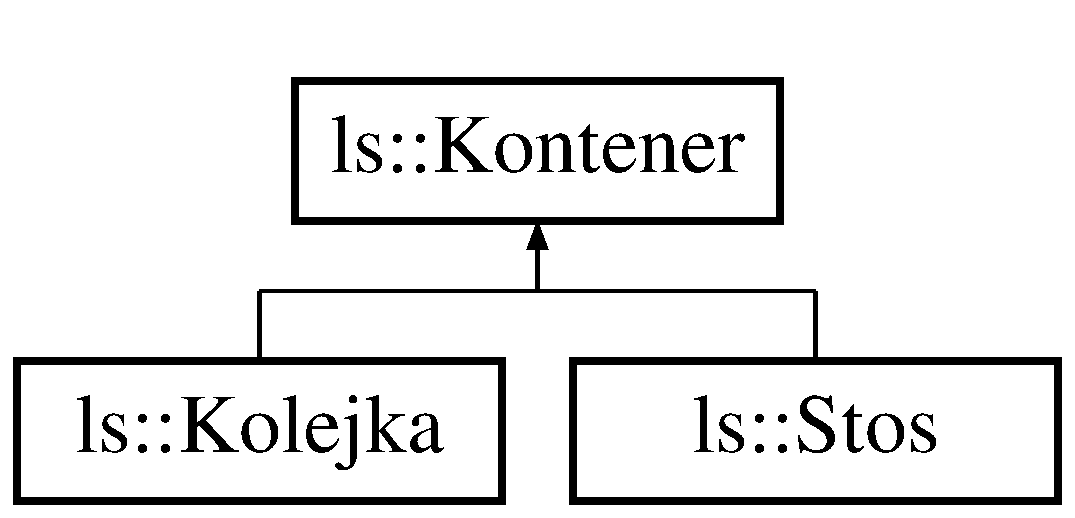
\includegraphics[height=2.000000cm]{classls_1_1_kontener}
\end{center}
\end{figure}
\subsection*{Metody publiczne}
\begin{DoxyCompactItemize}
\item 
\hyperlink{classls_1_1_kontener_a52711b1bc80413d48840ce8071a427fa}{$\sim$\-Kontener} ()
\begin{DoxyCompactList}\small\item\em Konstruktor klasy \hyperlink{classls_1_1_kontener}{Kontener}. \end{DoxyCompactList}\item 
\hyperlink{classls_1_1_kontener_a1c8f0e384b9d8e945ee70354eb144657}{Kontener} ()
\item 
void \hyperlink{classls_1_1_kontener_a911b275202510df1f321f8da26f0aa34}{push} (int)
\begin{DoxyCompactList}\small\item\em Wrzuca nową cegiełkę na początek kontenera. \end{DoxyCompactList}\item 
void \hyperlink{classls_1_1_kontener_a09517b6ec268d37744b1abbc7b7df5bb}{insert} (int wartosc, int indeks)
\begin{DoxyCompactList}\small\item\em Umieszcza cegłę z wartością 'wartosc' w miejscu oddalonym o 'indeks' miejsc od początku kontenera. \end{DoxyCompactList}\item 
int \hyperlink{classls_1_1_kontener_a248ac01db2477296b265fb0ea07a8c1c}{size} ()
\begin{DoxyCompactList}\small\item\em Liczy z ilu cegiełek składa się kontener. \end{DoxyCompactList}\item 
int \hyperlink{classls_1_1_kontener_a3b9fed0ce54e6232bd2868bf4b3801ec}{erase} (int)
\begin{DoxyCompactList}\small\item\em Usuwa z listy element o wybranym indeksie. \end{DoxyCompactList}\item 
int \hyperlink{classls_1_1_kontener_a04841df56a29d488e5e0d1a292646dde}{find} (int)
\begin{DoxyCompactList}\small\item\em Odnajduje w kontenerze przekazaną w argumencie wartość. \end{DoxyCompactList}\item 
void \hyperlink{classls_1_1_kontener_a75014b0a40e25ac573e2242d50522e08}{show} ()
\begin{DoxyCompactList}\small\item\em Wypisuje elementy listy od najmłodszego zaczynając. \end{DoxyCompactList}\end{DoxyCompactItemize}
\subsection*{Atrybuty chronione}
\begin{DoxyCompactItemize}
\item 
\hyperlink{structcegla}{cegla} $\ast$ \hyperlink{classls_1_1_kontener_af14ba3415f7ed315583ccb4575dfed9f}{alfa}
\end{DoxyCompactItemize}


\subsection{Opis szczegółowy}


Definicja w linii 14 pliku kontener.\-h.



\subsection{Dokumentacja konstruktora i destruktora}
\hypertarget{classls_1_1_kontener_a52711b1bc80413d48840ce8071a427fa}{\index{ls\-::\-Kontener@{ls\-::\-Kontener}!$\sim$\-Kontener@{$\sim$\-Kontener}}
\index{$\sim$\-Kontener@{$\sim$\-Kontener}!ls::Kontener@{ls\-::\-Kontener}}
\subsubsection[{$\sim$\-Kontener}]{\setlength{\rightskip}{0pt plus 5cm}ls\-::\-Kontener\-::$\sim$\-Kontener (
\begin{DoxyParamCaption}
{}
\end{DoxyParamCaption}
)}}\label{classls_1_1_kontener_a52711b1bc80413d48840ce8071a427fa}
Konstruktor klasy \hyperlink{classls_1_1_kontener}{Kontener} inicjalizuje wskaźnik 'alfa' wartością N\-U\-L\-L. 

Definicja w linii 7 pliku kontener.\-cpp.

\hypertarget{classls_1_1_kontener_a1c8f0e384b9d8e945ee70354eb144657}{\index{ls\-::\-Kontener@{ls\-::\-Kontener}!Kontener@{Kontener}}
\index{Kontener@{Kontener}!ls::Kontener@{ls\-::\-Kontener}}
\subsubsection[{Kontener}]{\setlength{\rightskip}{0pt plus 5cm}ls\-::\-Kontener\-::\-Kontener (
\begin{DoxyParamCaption}
{}
\end{DoxyParamCaption}
)\hspace{0.3cm}{\ttfamily [inline]}}}\label{classls_1_1_kontener_a1c8f0e384b9d8e945ee70354eb144657}


Definicja w linii 27 pliku kontener.\-h.



\subsection{Dokumentacja funkcji składowych}
\hypertarget{classls_1_1_kontener_a3b9fed0ce54e6232bd2868bf4b3801ec}{\index{ls\-::\-Kontener@{ls\-::\-Kontener}!erase@{erase}}
\index{erase@{erase}!ls::Kontener@{ls\-::\-Kontener}}
\subsubsection[{erase}]{\setlength{\rightskip}{0pt plus 5cm}int ls\-::\-Kontener\-::erase (
\begin{DoxyParamCaption}
\item[{int}]{indeks}
\end{DoxyParamCaption}
)}}\label{classls_1_1_kontener_a3b9fed0ce54e6232bd2868bf4b3801ec}
Zainicjalizowane są dwa wskaźniki na najmłodszą cegiełkę. Jeden jest ustawiany na element do usunięcia, drugi na element o jeden młodszy. Następuje roszada wskaźników\-: wskaźnik młodszej cegły wskazuje na cegłę starszą od usuwanej, zostaje zapisana wartość przechowywana przez usuwaną cegłę i wreszcie zwolniona zostaje pamięć zajmowana dotychczas przez cegłę.

Przykład 1\-: Wyrażenie obj.\-erase(0) usuwa najmłodszy element kontenera. Przykład 2\-: Wyrażenie obj.\-erase(obj.\-size() -\/ 1) usuwa najstarszy element. Przykład 3\-: Wyrażenie obj.\-erase(obj.\-size()) nie zmienia kontenera.

\begin{DoxyReturn}{Zwraca}
Zwraca wartość przechowywaną w usuniętej cegiełce. 
\end{DoxyReturn}


Definicja w linii 65 pliku kontener.\-cpp.

\hypertarget{classls_1_1_kontener_a04841df56a29d488e5e0d1a292646dde}{\index{ls\-::\-Kontener@{ls\-::\-Kontener}!find@{find}}
\index{find@{find}!ls::Kontener@{ls\-::\-Kontener}}
\subsubsection[{find}]{\setlength{\rightskip}{0pt plus 5cm}int ls\-::\-Kontener\-::find (
\begin{DoxyParamCaption}
\item[{int}]{wartosc}
\end{DoxyParamCaption}
)}}\label{classls_1_1_kontener_a04841df56a29d488e5e0d1a292646dde}
Powołany do życia jest szpieg -\/ wskaźnik na obiekt typu 'cegla', który przemierza kontener w poszukiwaniu najwcześniejszego wystąpienia poszukiwanej wartości. Operacji towarzyszy licznik, który śledzi ilość miniętych przez wskaźnik cegieł, którą metoda zwraca. Należy ją interpretować jako indeks cegły, gdzie najwcześniej wystąpiła poszukiwana wartość.

\begin{DoxyReturn}{Zwraca}
Zwraca indeks (liczony od 0 od najmłodszej cegiełki) najbliższego wystąpienia poszukiwanej wartości. 
\end{DoxyReturn}


Definicja w linii 99 pliku kontener.\-cpp.

\hypertarget{classls_1_1_kontener_a09517b6ec268d37744b1abbc7b7df5bb}{\index{ls\-::\-Kontener@{ls\-::\-Kontener}!insert@{insert}}
\index{insert@{insert}!ls::Kontener@{ls\-::\-Kontener}}
\subsubsection[{insert}]{\setlength{\rightskip}{0pt plus 5cm}void ls\-::\-Kontener\-::insert (
\begin{DoxyParamCaption}
\item[{int}]{wartosc, }
\item[{int}]{indeks}
\end{DoxyParamCaption}
)}}\label{classls_1_1_kontener_a09517b6ec268d37744b1abbc7b7df5bb}
U\-W\-A\-G\-A\-: Indeks liczony jest od zera, od najmłodszej cegły.

Przykład 1\-: Wyrażenie obj.\-insert(5,0) jest równoważne wyrażeniu obj.\-push(5)
\begin{DoxyItemize}
\item element zawierający wartość 5 jest teraz najmłodszym elementem. Przykład 2\-: Wyrażenie obj.\-insert(3,obj.\-size()) czyni element zawierający wartosć 3 najstarszym elementem. 
\end{DoxyItemize}

Definicja w linii 21 pliku kontener.\-cpp.

\hypertarget{classls_1_1_kontener_a911b275202510df1f321f8da26f0aa34}{\index{ls\-::\-Kontener@{ls\-::\-Kontener}!push@{push}}
\index{push@{push}!ls::Kontener@{ls\-::\-Kontener}}
\subsubsection[{push}]{\setlength{\rightskip}{0pt plus 5cm}void ls\-::\-Kontener\-::push (
\begin{DoxyParamCaption}
\item[{int}]{wart}
\end{DoxyParamCaption}
)}}\label{classls_1_1_kontener_a911b275202510df1f321f8da26f0aa34}


Definicja w linii 13 pliku kontener.\-cpp.

\hypertarget{classls_1_1_kontener_a75014b0a40e25ac573e2242d50522e08}{\index{ls\-::\-Kontener@{ls\-::\-Kontener}!show@{show}}
\index{show@{show}!ls::Kontener@{ls\-::\-Kontener}}
\subsubsection[{show}]{\setlength{\rightskip}{0pt plus 5cm}void ls\-::\-Kontener\-::show (
\begin{DoxyParamCaption}
{}
\end{DoxyParamCaption}
)}}\label{classls_1_1_kontener_a75014b0a40e25ac573e2242d50522e08}


Definicja w linii 116 pliku kontener.\-cpp.

\hypertarget{classls_1_1_kontener_a248ac01db2477296b265fb0ea07a8c1c}{\index{ls\-::\-Kontener@{ls\-::\-Kontener}!size@{size}}
\index{size@{size}!ls::Kontener@{ls\-::\-Kontener}}
\subsubsection[{size}]{\setlength{\rightskip}{0pt plus 5cm}int ls\-::\-Kontener\-::size (
\begin{DoxyParamCaption}
{}
\end{DoxyParamCaption}
)}}\label{classls_1_1_kontener_a248ac01db2477296b265fb0ea07a8c1c}
Zainicjalizowany zostaje wskaźnik na strukturę 'cegla' wskazujący na najmłodszą cegiełkę. Zostaje on potem wysłany w epicką podróż na sam koniec kontenera (czyli do napotkania N\-U\-L\-La). Towarzyszy mu licznik, który zlicza mijane po drodze cegiełki, których ilosć funkcja zwraca.

\begin{DoxyReturn}{Zwraca}
Zwraca wielkość kontenera. 
\end{DoxyReturn}


Definicja w linii 50 pliku kontener.\-cpp.



\subsection{Dokumentacja atrybutów składowych}
\hypertarget{classls_1_1_kontener_af14ba3415f7ed315583ccb4575dfed9f}{\index{ls\-::\-Kontener@{ls\-::\-Kontener}!alfa@{alfa}}
\index{alfa@{alfa}!ls::Kontener@{ls\-::\-Kontener}}
\subsubsection[{alfa}]{\setlength{\rightskip}{0pt plus 5cm}{\bf cegla}$\ast$ ls\-::\-Kontener\-::alfa\hspace{0.3cm}{\ttfamily [protected]}}}\label{classls_1_1_kontener_af14ba3415f7ed315583ccb4575dfed9f}


Definicja w linii 17 pliku kontener.\-h.



Dokumentacja dla tej klasy została wygenerowana z plików\-:\begin{DoxyCompactItemize}
\item 
\hyperlink{kontener_8h}{kontener.\-h}\item 
\hyperlink{kontener_8cpp}{kontener.\-cpp}\end{DoxyCompactItemize}

\hypertarget{classarr_1_1_lista}{\section{Dokumentacja klasy arr\-:\-:Lista}
\label{classarr_1_1_lista}\index{arr\-::\-Lista@{arr\-::\-Lista}}
}


{\ttfamily \#include $<$lista\-\_\-arr.\-h$>$}

\subsection*{Metody publiczne}
\begin{DoxyCompactItemize}
\item 
\hyperlink{classarr_1_1_lista_a11b61b647380e962aeeb35848c427b81}{Lista} ()
\begin{DoxyCompactList}\small\item\em Konstruktor domyślny klasy \hyperlink{classarr_1_1_lista}{arr\-::\-Lista}. \end{DoxyCompactList}\item 
\hyperlink{classarr_1_1_lista_a29bae0190a2d5c38ebfdf33eb05d1c09}{Lista} (const \hyperlink{classarr_1_1_lista}{Lista} \&lewy)
\begin{DoxyCompactList}\small\item\em Konstruktor kopiujący klasy \hyperlink{classarr_1_1_lista}{arr\-::\-Lista}. \end{DoxyCompactList}\item 
\hyperlink{classarr_1_1_lista_ac3b5f77b08befbf28e922179dcace594}{$\sim$\-Lista} ()
\begin{DoxyCompactList}\small\item\em Destruktor klasy \hyperlink{classarr_1_1_lista}{arr\-::\-Lista}. \end{DoxyCompactList}\item 
int \hyperlink{classarr_1_1_lista_ad370aa7f4e6bf3f2492f5187c9d64d56}{erase} (int)
\begin{DoxyCompactList}\small\item\em Usuwa z listy element o wybranym indeksie. \end{DoxyCompactList}\item 
void \hyperlink{classarr_1_1_lista_a57365c410ba6ac9d82eb4b4a83bc89bd}{insert} (int, int)
\begin{DoxyCompactList}\small\item\em Umieszcza cegłę z wartością 'wartosc' w miejscu oddalonym o 'indeks' miejsc od początku kontenera. \end{DoxyCompactList}\item 
bool \hyperlink{classarr_1_1_lista_a6eef5db974ccbb5f133a76d22b375ae9}{empty} ()
\begin{DoxyCompactList}\small\item\em Sprawdza, czy lista jest pusta. \end{DoxyCompactList}\item 
int \hyperlink{classarr_1_1_lista_a853418a2061e80c83185f03f0e1568c6}{size} ()
\begin{DoxyCompactList}\small\item\em Zwraca rozmiar listy. \end{DoxyCompactList}\end{DoxyCompactItemize}
\subsection*{Metody prywatne}
\begin{DoxyCompactItemize}
\item 
void \hyperlink{classarr_1_1_lista_ac4f01715efe075f780e006d757ed0c26}{rozszerz\-\_\-x2} ()
\begin{DoxyCompactList}\small\item\em Metoda zwiększa dwukrotnie pojemnosć listy. \end{DoxyCompactList}\item 
void \hyperlink{classarr_1_1_lista_ad6bf8061555507002920efbe6f3c0bb1}{rozszerz\-\_\-1} ()
\begin{DoxyCompactList}\small\item\em Metoda zwiększa pojemnosć listy o 1. \end{DoxyCompactList}\end{DoxyCompactItemize}
\subsection*{Atrybuty prywatne}
\begin{DoxyCompactItemize}
\item 
int $\ast$ \hyperlink{classarr_1_1_lista_aba76002ee48a3dc21187f0bf9da1a746}{tablica}
\item 
int \hyperlink{classarr_1_1_lista_a5d6712accdb4a0eda72038aadbfe1cd6}{rozmiar\-\_\-ls}
\item 
int \hyperlink{classarr_1_1_lista_a46550171712501ae7301b95b5c35d14c}{pojemnosc\-\_\-ls}
\end{DoxyCompactItemize}


\subsection{Opis szczegółowy}


Definicja w linii 6 pliku lista\-\_\-arr.\-h.



\subsection{Dokumentacja konstruktora i destruktora}
\hypertarget{classarr_1_1_lista_a11b61b647380e962aeeb35848c427b81}{\index{arr\-::\-Lista@{arr\-::\-Lista}!Lista@{Lista}}
\index{Lista@{Lista}!arr::Lista@{arr\-::\-Lista}}
\subsubsection[{Lista}]{\setlength{\rightskip}{0pt plus 5cm}arr\-::\-Lista\-::\-Lista (
\begin{DoxyParamCaption}
{}
\end{DoxyParamCaption}
)\hspace{0.3cm}{\ttfamily [inline]}}}\label{classarr_1_1_lista_a11b61b647380e962aeeb35848c427b81}


Definicja w linii 25 pliku lista\-\_\-arr.\-h.

\hypertarget{classarr_1_1_lista_a29bae0190a2d5c38ebfdf33eb05d1c09}{\index{arr\-::\-Lista@{arr\-::\-Lista}!Lista@{Lista}}
\index{Lista@{Lista}!arr::Lista@{arr\-::\-Lista}}
\subsubsection[{Lista}]{\setlength{\rightskip}{0pt plus 5cm}arr\-::\-Lista\-::\-Lista (
\begin{DoxyParamCaption}
\item[{const {\bf Lista} \&}]{lewy}
\end{DoxyParamCaption}
)}}\label{classarr_1_1_lista_a29bae0190a2d5c38ebfdf33eb05d1c09}
Bezużyteczny dla trzeciego zadania, ale na pewno kolega się ucieszy. \hypertarget{classarr_1_1_lista_ac3b5f77b08befbf28e922179dcace594}{\index{arr\-::\-Lista@{arr\-::\-Lista}!$\sim$\-Lista@{$\sim$\-Lista}}
\index{$\sim$\-Lista@{$\sim$\-Lista}!arr::Lista@{arr\-::\-Lista}}
\subsubsection[{$\sim$\-Lista}]{\setlength{\rightskip}{0pt plus 5cm}arr\-::\-Lista\-::$\sim$\-Lista (
\begin{DoxyParamCaption}
{}
\end{DoxyParamCaption}
)\hspace{0.3cm}{\ttfamily [inline]}}}\label{classarr_1_1_lista_ac3b5f77b08befbf28e922179dcace594}


Definicja w linii 35 pliku lista\-\_\-arr.\-h.



\subsection{Dokumentacja funkcji składowych}
\hypertarget{classarr_1_1_lista_a6eef5db974ccbb5f133a76d22b375ae9}{\index{arr\-::\-Lista@{arr\-::\-Lista}!empty@{empty}}
\index{empty@{empty}!arr::Lista@{arr\-::\-Lista}}
\subsubsection[{empty}]{\setlength{\rightskip}{0pt plus 5cm}bool arr\-::\-Lista\-::empty (
\begin{DoxyParamCaption}
{}
\end{DoxyParamCaption}
)}}\label{classarr_1_1_lista_a6eef5db974ccbb5f133a76d22b375ae9}
\begin{DoxyReturn}{Zwraca}
Zwraca prawdę, jeżeli lista jest pusta. W przeciwnym razie zwraca false. 
\end{DoxyReturn}


Definicja w linii 3 pliku lista\-\_\-arr.\-cpp.

\hypertarget{classarr_1_1_lista_ad370aa7f4e6bf3f2492f5187c9d64d56}{\index{arr\-::\-Lista@{arr\-::\-Lista}!erase@{erase}}
\index{erase@{erase}!arr::Lista@{arr\-::\-Lista}}
\subsubsection[{erase}]{\setlength{\rightskip}{0pt plus 5cm}int arr\-::\-Lista\-::erase (
\begin{DoxyParamCaption}
\item[{int}]{indeks}
\end{DoxyParamCaption}
)}}\label{classarr_1_1_lista_ad370aa7f4e6bf3f2492f5187c9d64d56}
Zapisuje wartość przechowywaną pod danym indeksem a potem przesuwa całą zawartość tablicy młodszą od danego elementu o 1 w stronę starszych elementów. Zmniejsza licznik rozmiar\-\_\-ls o 1.

Przykład 1\-: Wyrażenie obj.\-erase(0) usuwa najmłodszy element kontenera. Przykład 2\-: Wyrażenie obj.\-erase(obj.\-size() -\/ 1) usuwa najstarszy element. Przykład 3\-: Wyrażenie obj.\-erase(obj.\-size()) nie zmienia kontenera.

\begin{DoxyReturn}{Zwraca}
Zwraca wartość przechowywaną w usuniętej cegiełce. 
\end{DoxyReturn}


Definicja w linii 8 pliku lista\-\_\-arr.\-cpp.

\hypertarget{classarr_1_1_lista_a57365c410ba6ac9d82eb4b4a83bc89bd}{\index{arr\-::\-Lista@{arr\-::\-Lista}!insert@{insert}}
\index{insert@{insert}!arr::Lista@{arr\-::\-Lista}}
\subsubsection[{insert}]{\setlength{\rightskip}{0pt plus 5cm}void arr\-::\-Lista\-::insert (
\begin{DoxyParamCaption}
\item[{int}]{value, }
\item[{int}]{indeks}
\end{DoxyParamCaption}
)}}\label{classarr_1_1_lista_a57365c410ba6ac9d82eb4b4a83bc89bd}
Zwiększa licznik rozmiar\-\_\-ls o 1, odsuwa wszystkie elementy młodsze od danego indeksu o 1 od starszych i umieszcza wartość w odpowiednim indeksie. Może powodować realokację zawartości listy!

U\-W\-A\-G\-A\-: Indeks liczony jest od zera, od najmłodszej cegły.

Przykład 1\-: Wyrażenie obj.\-insert(5,0) jest równoważne wyrażeniu obj.\-push(5)
\begin{DoxyItemize}
\item element zawierający wartość 5 jest teraz najmłodszym elementem. Przykład 2\-: Wyrażenie obj.\-insert(3,obj.\-size()) czyni element zawierający wartosć 3 najstarszym elementem. 
\end{DoxyItemize}

Definicja w linii 20 pliku lista\-\_\-arr.\-cpp.

\hypertarget{classarr_1_1_lista_ad6bf8061555507002920efbe6f3c0bb1}{\index{arr\-::\-Lista@{arr\-::\-Lista}!rozszerz\-\_\-1@{rozszerz\-\_\-1}}
\index{rozszerz\-\_\-1@{rozszerz\-\_\-1}!arr::Lista@{arr\-::\-Lista}}
\subsubsection[{rozszerz\-\_\-1}]{\setlength{\rightskip}{0pt plus 5cm}void arr\-::\-Lista\-::rozszerz\-\_\-1 (
\begin{DoxyParamCaption}
{}
\end{DoxyParamCaption}
)\hspace{0.3cm}{\ttfamily [private]}}}\label{classarr_1_1_lista_ad6bf8061555507002920efbe6f3c0bb1}


Definicja w linii 59 pliku lista\-\_\-arr.\-cpp.

\hypertarget{classarr_1_1_lista_ac4f01715efe075f780e006d757ed0c26}{\index{arr\-::\-Lista@{arr\-::\-Lista}!rozszerz\-\_\-x2@{rozszerz\-\_\-x2}}
\index{rozszerz\-\_\-x2@{rozszerz\-\_\-x2}!arr::Lista@{arr\-::\-Lista}}
\subsubsection[{rozszerz\-\_\-x2}]{\setlength{\rightskip}{0pt plus 5cm}void arr\-::\-Lista\-::rozszerz\-\_\-x2 (
\begin{DoxyParamCaption}
{}
\end{DoxyParamCaption}
)\hspace{0.3cm}{\ttfamily [private]}}}\label{classarr_1_1_lista_ac4f01715efe075f780e006d757ed0c26}


Definicja w linii 44 pliku lista\-\_\-arr.\-cpp.

\hypertarget{classarr_1_1_lista_a853418a2061e80c83185f03f0e1568c6}{\index{arr\-::\-Lista@{arr\-::\-Lista}!size@{size}}
\index{size@{size}!arr::Lista@{arr\-::\-Lista}}
\subsubsection[{size}]{\setlength{\rightskip}{0pt plus 5cm}int arr\-::\-Lista\-::size (
\begin{DoxyParamCaption}
{}
\end{DoxyParamCaption}
)\hspace{0.3cm}{\ttfamily [inline]}}}\label{classarr_1_1_lista_a853418a2061e80c83185f03f0e1568c6}


Definicja w linii 83 pliku lista\-\_\-arr.\-h.



\subsection{Dokumentacja atrybutów składowych}
\hypertarget{classarr_1_1_lista_a46550171712501ae7301b95b5c35d14c}{\index{arr\-::\-Lista@{arr\-::\-Lista}!pojemnosc\-\_\-ls@{pojemnosc\-\_\-ls}}
\index{pojemnosc\-\_\-ls@{pojemnosc\-\_\-ls}!arr::Lista@{arr\-::\-Lista}}
\subsubsection[{pojemnosc\-\_\-ls}]{\setlength{\rightskip}{0pt plus 5cm}int arr\-::\-Lista\-::pojemnosc\-\_\-ls\hspace{0.3cm}{\ttfamily [private]}}}\label{classarr_1_1_lista_a46550171712501ae7301b95b5c35d14c}


Definicja w linii 11 pliku lista\-\_\-arr.\-h.

\hypertarget{classarr_1_1_lista_a5d6712accdb4a0eda72038aadbfe1cd6}{\index{arr\-::\-Lista@{arr\-::\-Lista}!rozmiar\-\_\-ls@{rozmiar\-\_\-ls}}
\index{rozmiar\-\_\-ls@{rozmiar\-\_\-ls}!arr::Lista@{arr\-::\-Lista}}
\subsubsection[{rozmiar\-\_\-ls}]{\setlength{\rightskip}{0pt plus 5cm}int arr\-::\-Lista\-::rozmiar\-\_\-ls\hspace{0.3cm}{\ttfamily [private]}}}\label{classarr_1_1_lista_a5d6712accdb4a0eda72038aadbfe1cd6}


Definicja w linii 10 pliku lista\-\_\-arr.\-h.

\hypertarget{classarr_1_1_lista_aba76002ee48a3dc21187f0bf9da1a746}{\index{arr\-::\-Lista@{arr\-::\-Lista}!tablica@{tablica}}
\index{tablica@{tablica}!arr::Lista@{arr\-::\-Lista}}
\subsubsection[{tablica}]{\setlength{\rightskip}{0pt plus 5cm}int$\ast$ arr\-::\-Lista\-::tablica\hspace{0.3cm}{\ttfamily [private]}}}\label{classarr_1_1_lista_aba76002ee48a3dc21187f0bf9da1a746}


Definicja w linii 9 pliku lista\-\_\-arr.\-h.



Dokumentacja dla tej klasy została wygenerowana z plików\-:\begin{DoxyCompactItemize}
\item 
\hyperlink{lista__arr_8h}{lista\-\_\-arr.\-h}\item 
\hyperlink{lista__arr_8cpp}{lista\-\_\-arr.\-cpp}\end{DoxyCompactItemize}

\hypertarget{classls_1_1_stos}{\section{Dokumentacja klasy ls\-:\-:Stos}
\label{classls_1_1_stos}\index{ls\-::\-Stos@{ls\-::\-Stos}}
}


{\ttfamily \#include $<$stos.\-h$>$}

Diagram dziedziczenia dla ls\-:\-:Stos\begin{figure}[H]
\begin{center}
\leavevmode
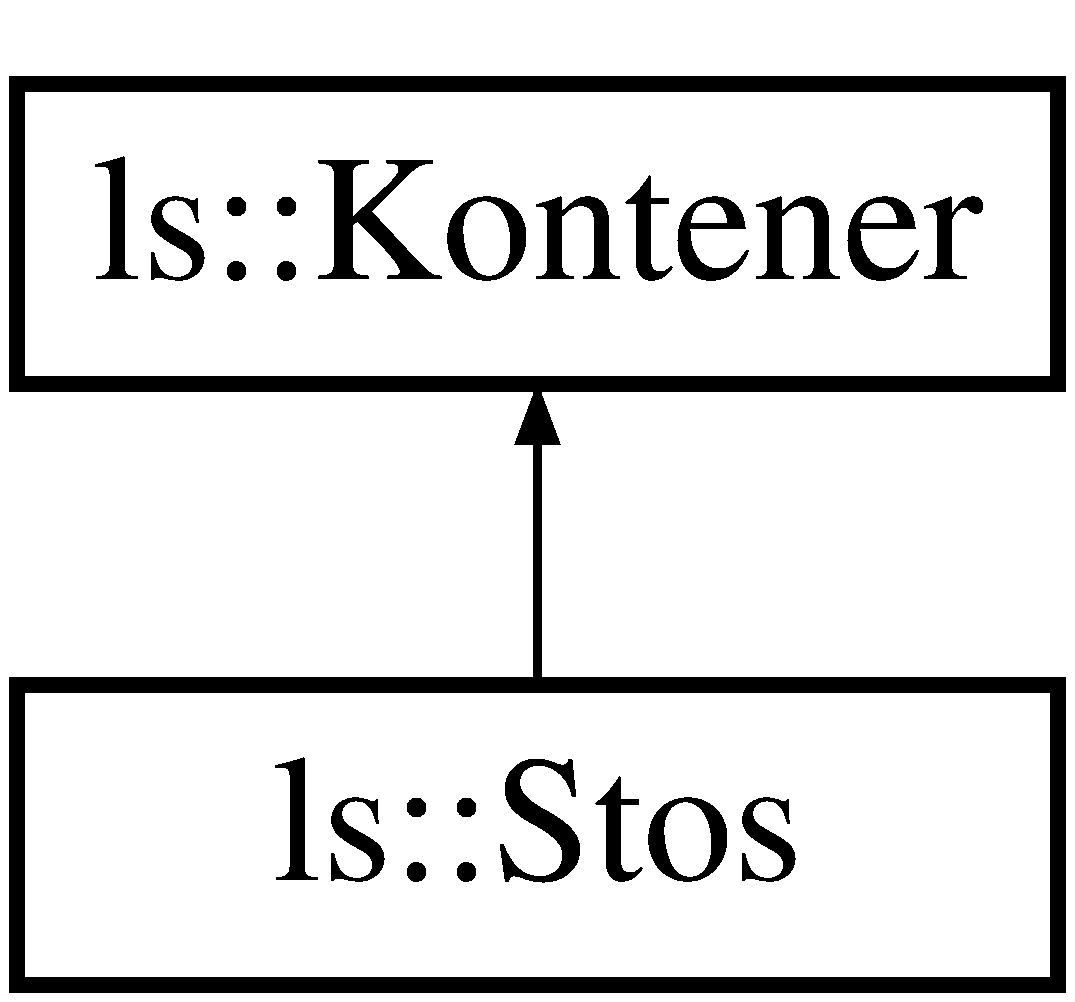
\includegraphics[height=2.000000cm]{classls_1_1_stos}
\end{center}
\end{figure}
\subsection*{Metody publiczne}
\begin{DoxyCompactItemize}
\item 
\hyperlink{classls_1_1_stos_a600e24b908c21f945c451066f84b0bc4}{$\sim$\-Stos} ()
\item 
int \hyperlink{classls_1_1_stos_aba0c11a34e5018a1e96b4822de2c2dfc}{pop} ()
\begin{DoxyCompactList}\small\item\em Pop stosu jaki jest, każdy widzi. Zdejmuje najmłdoszy element i zwraca wartość przez niego przechowywaną. \end{DoxyCompactList}\end{DoxyCompactItemize}
\subsection*{Dodatkowe Dziedziczone Składowe}


\subsection{Opis szczegółowy}


Definicja w linii 14 pliku stos.\-h.



\subsection{Dokumentacja konstruktora i destruktora}
\hypertarget{classls_1_1_stos_a600e24b908c21f945c451066f84b0bc4}{\index{ls\-::\-Stos@{ls\-::\-Stos}!$\sim$\-Stos@{$\sim$\-Stos}}
\index{$\sim$\-Stos@{$\sim$\-Stos}!ls::Stos@{ls\-::\-Stos}}
\subsubsection[{$\sim$\-Stos}]{\setlength{\rightskip}{0pt plus 5cm}ls\-::\-Stos\-::$\sim$\-Stos (
\begin{DoxyParamCaption}
{}
\end{DoxyParamCaption}
)\hspace{0.3cm}{\ttfamily [inline]}}}\label{classls_1_1_stos_a600e24b908c21f945c451066f84b0bc4}


Definicja w linii 17 pliku stos.\-h.



\subsection{Dokumentacja funkcji składowych}
\hypertarget{classls_1_1_stos_aba0c11a34e5018a1e96b4822de2c2dfc}{\index{ls\-::\-Stos@{ls\-::\-Stos}!pop@{pop}}
\index{pop@{pop}!ls::Stos@{ls\-::\-Stos}}
\subsubsection[{pop}]{\setlength{\rightskip}{0pt plus 5cm}int ls\-::\-Stos\-::pop (
\begin{DoxyParamCaption}
{}
\end{DoxyParamCaption}
)\hspace{0.3cm}{\ttfamily [inline]}}}\label{classls_1_1_stos_aba0c11a34e5018a1e96b4822de2c2dfc}


Definicja w linii 25 pliku stos.\-h.



Dokumentacja dla tej klasy została wygenerowana z pliku\-:\begin{DoxyCompactItemize}
\item 
\hyperlink{stos_8h}{stos.\-h}\end{DoxyCompactItemize}

\hypertarget{classarr_1_1_stos}{\section{Dokumentacja klasy arr\-:\-:Stos}
\label{classarr_1_1_stos}\index{arr\-::\-Stos@{arr\-::\-Stos}}
}


{\ttfamily \#include $<$stos\-\_\-arr.\-h$>$}

\subsection*{Metody publiczne}
\begin{DoxyCompactItemize}
\item 
\hyperlink{classarr_1_1_stos_acc173736bd233091fe1205c7b2ad08e3}{Stos} ()
\begin{DoxyCompactList}\small\item\em Konstruktor domyślny klasy \hyperlink{classarr_1_1_stos}{Stos}. \end{DoxyCompactList}\item 
\hyperlink{classarr_1_1_stos_a3fa4c0909a0a8af714a7a41925c9bfc4}{Stos} (const \hyperlink{classarr_1_1_stos}{Stos} \&lewy)
\begin{DoxyCompactList}\small\item\em Konstruktor kopiujący klasy \hyperlink{classarr_1_1_stos}{Stos}. \end{DoxyCompactList}\item 
\hyperlink{classarr_1_1_stos_aab930de62382058082057237c0651c85}{$\sim$\-Stos} ()
\begin{DoxyCompactList}\small\item\em Destruktor klasy \hyperlink{classarr_1_1_stos}{Stos}. \end{DoxyCompactList}\item 
void \hyperlink{classarr_1_1_stos_a818b45b7e1133cf8666a8996795823a6}{push} (int val)
\begin{DoxyCompactList}\small\item\em Wrzuca element na szczyt stosu. \end{DoxyCompactList}\item 
int \hyperlink{classarr_1_1_stos_a3d8fd4cebbcc8eb5aed6bfe15e1b86d8}{pop} ()
\begin{DoxyCompactList}\small\item\em Zdejmuje najmłodszy element ze stosu. \end{DoxyCompactList}\item 
bool \hyperlink{classarr_1_1_stos_aa65aee46af4fbfe791b7419d9e2dc2d1}{empty} ()
\begin{DoxyCompactList}\small\item\em Sprawdza, czy stos jest pusty. \end{DoxyCompactList}\item 
int \hyperlink{classarr_1_1_stos_a7f40cb3055b25794dfd484e6e8bd4822}{size} ()
\begin{DoxyCompactList}\small\item\em Zwraca rozmiar stosu. \end{DoxyCompactList}\end{DoxyCompactItemize}
\subsection*{Metody prywatne}
\begin{DoxyCompactItemize}
\item 
void \hyperlink{classarr_1_1_stos_a26833a56e91aefa4dfbc78cafe7ef216}{rozszerz\-\_\-x2} ()
\begin{DoxyCompactList}\small\item\em Metoda zwiększa dwukrotnie pojemnosć stosu. \end{DoxyCompactList}\item 
void \hyperlink{classarr_1_1_stos_a302eb8f0ef06039bd7408a881d3d2c60}{rozszerz\-\_\-1} ()
\begin{DoxyCompactList}\small\item\em Metoda zwiększa pojemnosć stosu o 1. \end{DoxyCompactList}\end{DoxyCompactItemize}
\subsection*{Atrybuty prywatne}
\begin{DoxyCompactItemize}
\item 
int $\ast$ \hyperlink{classarr_1_1_stos_ad8e05da5f97f966b3c4f21d661e88b05}{tablica}
\item 
int \hyperlink{classarr_1_1_stos_a1980b721d3a83d8811b07ccf37f62e5e}{rozmiar\-\_\-stosu}
\item 
int \hyperlink{classarr_1_1_stos_a577c49248d0925cb5ca4f0a53aeebe8c}{pojemnosc\-\_\-stosu}
\end{DoxyCompactItemize}


\subsection{Opis szczegółowy}


Definicja w linii 7 pliku stos\-\_\-arr.\-h.



\subsection{Dokumentacja konstruktora i destruktora}
\hypertarget{classarr_1_1_stos_acc173736bd233091fe1205c7b2ad08e3}{\index{arr\-::\-Stos@{arr\-::\-Stos}!Stos@{Stos}}
\index{Stos@{Stos}!arr::Stos@{arr\-::\-Stos}}
\subsubsection[{Stos}]{\setlength{\rightskip}{0pt plus 5cm}arr\-::\-Stos\-::\-Stos (
\begin{DoxyParamCaption}
{}
\end{DoxyParamCaption}
)\hspace{0.3cm}{\ttfamily [inline]}}}\label{classarr_1_1_stos_acc173736bd233091fe1205c7b2ad08e3}


Definicja w linii 26 pliku stos\-\_\-arr.\-h.

\hypertarget{classarr_1_1_stos_a3fa4c0909a0a8af714a7a41925c9bfc4}{\index{arr\-::\-Stos@{arr\-::\-Stos}!Stos@{Stos}}
\index{Stos@{Stos}!arr::Stos@{arr\-::\-Stos}}
\subsubsection[{Stos}]{\setlength{\rightskip}{0pt plus 5cm}arr\-::\-Stos\-::\-Stos (
\begin{DoxyParamCaption}
\item[{const {\bf Stos} \&}]{lewy}
\end{DoxyParamCaption}
)}}\label{classarr_1_1_stos_a3fa4c0909a0a8af714a7a41925c9bfc4}
Bezużyteczny dla trzeciego zadania, ale na pewno kolega się ucieszy. 

Definicja w linii 3 pliku stos\-\_\-arr.\-cpp.

\hypertarget{classarr_1_1_stos_aab930de62382058082057237c0651c85}{\index{arr\-::\-Stos@{arr\-::\-Stos}!$\sim$\-Stos@{$\sim$\-Stos}}
\index{$\sim$\-Stos@{$\sim$\-Stos}!arr::Stos@{arr\-::\-Stos}}
\subsubsection[{$\sim$\-Stos}]{\setlength{\rightskip}{0pt plus 5cm}arr\-::\-Stos\-::$\sim$\-Stos (
\begin{DoxyParamCaption}
{}
\end{DoxyParamCaption}
)}}\label{classarr_1_1_stos_aab930de62382058082057237c0651c85}


Definicja w linii 10 pliku stos\-\_\-arr.\-cpp.



\subsection{Dokumentacja funkcji składowych}
\hypertarget{classarr_1_1_stos_aa65aee46af4fbfe791b7419d9e2dc2d1}{\index{arr\-::\-Stos@{arr\-::\-Stos}!empty@{empty}}
\index{empty@{empty}!arr::Stos@{arr\-::\-Stos}}
\subsubsection[{empty}]{\setlength{\rightskip}{0pt plus 5cm}bool arr\-::\-Stos\-::empty (
\begin{DoxyParamCaption}
{}
\end{DoxyParamCaption}
)}}\label{classarr_1_1_stos_aa65aee46af4fbfe791b7419d9e2dc2d1}
\begin{DoxyReturn}{Zwraca}
Zwraca prawdę, jeżeli kolejka jest pusta. W przeciwnym razie zwraca false. 
\end{DoxyReturn}


Definicja w linii 38 pliku stos\-\_\-arr.\-cpp.

\hypertarget{classarr_1_1_stos_a3d8fd4cebbcc8eb5aed6bfe15e1b86d8}{\index{arr\-::\-Stos@{arr\-::\-Stos}!pop@{pop}}
\index{pop@{pop}!arr::Stos@{arr\-::\-Stos}}
\subsubsection[{pop}]{\setlength{\rightskip}{0pt plus 5cm}int arr\-::\-Stos\-::pop (
\begin{DoxyParamCaption}
{}
\end{DoxyParamCaption}
)}}\label{classarr_1_1_stos_a3d8fd4cebbcc8eb5aed6bfe15e1b86d8}


Definicja w linii 32 pliku stos\-\_\-arr.\-cpp.

\hypertarget{classarr_1_1_stos_a818b45b7e1133cf8666a8996795823a6}{\index{arr\-::\-Stos@{arr\-::\-Stos}!push@{push}}
\index{push@{push}!arr::Stos@{arr\-::\-Stos}}
\subsubsection[{push}]{\setlength{\rightskip}{0pt plus 5cm}void arr\-::\-Stos\-::push (
\begin{DoxyParamCaption}
\item[{int}]{val}
\end{DoxyParamCaption}
)}}\label{classarr_1_1_stos_a818b45b7e1133cf8666a8996795823a6}


Definicja w linii 15 pliku stos\-\_\-arr.\-cpp.

\hypertarget{classarr_1_1_stos_a302eb8f0ef06039bd7408a881d3d2c60}{\index{arr\-::\-Stos@{arr\-::\-Stos}!rozszerz\-\_\-1@{rozszerz\-\_\-1}}
\index{rozszerz\-\_\-1@{rozszerz\-\_\-1}!arr::Stos@{arr\-::\-Stos}}
\subsubsection[{rozszerz\-\_\-1}]{\setlength{\rightskip}{0pt plus 5cm}void arr\-::\-Stos\-::rozszerz\-\_\-1 (
\begin{DoxyParamCaption}
{}
\end{DoxyParamCaption}
)\hspace{0.3cm}{\ttfamily [private]}}}\label{classarr_1_1_stos_a302eb8f0ef06039bd7408a881d3d2c60}


Definicja w linii 58 pliku stos\-\_\-arr.\-cpp.

\hypertarget{classarr_1_1_stos_a26833a56e91aefa4dfbc78cafe7ef216}{\index{arr\-::\-Stos@{arr\-::\-Stos}!rozszerz\-\_\-x2@{rozszerz\-\_\-x2}}
\index{rozszerz\-\_\-x2@{rozszerz\-\_\-x2}!arr::Stos@{arr\-::\-Stos}}
\subsubsection[{rozszerz\-\_\-x2}]{\setlength{\rightskip}{0pt plus 5cm}void arr\-::\-Stos\-::rozszerz\-\_\-x2 (
\begin{DoxyParamCaption}
{}
\end{DoxyParamCaption}
)\hspace{0.3cm}{\ttfamily [private]}}}\label{classarr_1_1_stos_a26833a56e91aefa4dfbc78cafe7ef216}


Definicja w linii 43 pliku stos\-\_\-arr.\-cpp.

\hypertarget{classarr_1_1_stos_a7f40cb3055b25794dfd484e6e8bd4822}{\index{arr\-::\-Stos@{arr\-::\-Stos}!size@{size}}
\index{size@{size}!arr::Stos@{arr\-::\-Stos}}
\subsubsection[{size}]{\setlength{\rightskip}{0pt plus 5cm}int arr\-::\-Stos\-::size (
\begin{DoxyParamCaption}
{}
\end{DoxyParamCaption}
)\hspace{0.3cm}{\ttfamily [inline]}}}\label{classarr_1_1_stos_a7f40cb3055b25794dfd484e6e8bd4822}


Definicja w linii 54 pliku stos\-\_\-arr.\-h.



\subsection{Dokumentacja atrybutów składowych}
\hypertarget{classarr_1_1_stos_a577c49248d0925cb5ca4f0a53aeebe8c}{\index{arr\-::\-Stos@{arr\-::\-Stos}!pojemnosc\-\_\-stosu@{pojemnosc\-\_\-stosu}}
\index{pojemnosc\-\_\-stosu@{pojemnosc\-\_\-stosu}!arr::Stos@{arr\-::\-Stos}}
\subsubsection[{pojemnosc\-\_\-stosu}]{\setlength{\rightskip}{0pt plus 5cm}int arr\-::\-Stos\-::pojemnosc\-\_\-stosu\hspace{0.3cm}{\ttfamily [private]}}}\label{classarr_1_1_stos_a577c49248d0925cb5ca4f0a53aeebe8c}


Definicja w linii 12 pliku stos\-\_\-arr.\-h.

\hypertarget{classarr_1_1_stos_a1980b721d3a83d8811b07ccf37f62e5e}{\index{arr\-::\-Stos@{arr\-::\-Stos}!rozmiar\-\_\-stosu@{rozmiar\-\_\-stosu}}
\index{rozmiar\-\_\-stosu@{rozmiar\-\_\-stosu}!arr::Stos@{arr\-::\-Stos}}
\subsubsection[{rozmiar\-\_\-stosu}]{\setlength{\rightskip}{0pt plus 5cm}int arr\-::\-Stos\-::rozmiar\-\_\-stosu\hspace{0.3cm}{\ttfamily [private]}}}\label{classarr_1_1_stos_a1980b721d3a83d8811b07ccf37f62e5e}


Definicja w linii 11 pliku stos\-\_\-arr.\-h.

\hypertarget{classarr_1_1_stos_ad8e05da5f97f966b3c4f21d661e88b05}{\index{arr\-::\-Stos@{arr\-::\-Stos}!tablica@{tablica}}
\index{tablica@{tablica}!arr::Stos@{arr\-::\-Stos}}
\subsubsection[{tablica}]{\setlength{\rightskip}{0pt plus 5cm}int$\ast$ arr\-::\-Stos\-::tablica\hspace{0.3cm}{\ttfamily [private]}}}\label{classarr_1_1_stos_ad8e05da5f97f966b3c4f21d661e88b05}


Definicja w linii 10 pliku stos\-\_\-arr.\-h.



Dokumentacja dla tej klasy została wygenerowana z plików\-:\begin{DoxyCompactItemize}
\item 
\hyperlink{stos__arr_8h}{stos\-\_\-arr.\-h}\item 
\hyperlink{stos__arr_8cpp}{stos\-\_\-arr.\-cpp}\end{DoxyCompactItemize}

%--- End generated contents ---

% Index
\newpage
\phantomsection
\addcontentsline{toc}{chapter}{Indeks}
\printindex

\end{document}
